\documentclass[10pt]{report}
%\usepackage{fullpage}
\usepackage{graphicx}   % if you want to include graphics files
\usepackage{subfigure}
\usepackage{setspace}
\usepackage{amsxtra}
\usepackage{amsmath}
\usepackage{amssymb}
\usepackage{multirow}
\usepackage{algorithmic}
\usepackage{algorithm}

% graphics path
\graphicspath{{Figs/}}
%\usepackage{rotating}

%turns all margins to 1in
\addtolength{\oddsidemargin}{-.875in}
\addtolength{\evensidemargin}{-.875in}
\addtolength{\textwidth}{1.75in}

\addtolength{\topmargin}{-.875in}
\addtolength{\textheight}{1.75in}

\DeclareMathOperator{\sgn}{sgn} 
\setcounter{secnumdepth}{2}
\author{John Swoboda}
\title{\textbf{Incoherent Scatter Radar Simulator}}

\begin{document}
\maketitle

\chapter{Introduction}

This report covers the physics, and signal processing used to create the incoherent scatter radar (ISR) simulator that is in the code base. 

\chapter{ISR Spectrum}
\section*{Overview}

This is a description of the ISR spectrum process describes the mathematical basis for the software code base ISRSpectrum. It is based off of the development in  \cite{kudeki:milla:1} and \cite{Kudeki:2006kx} to form a spectrum.

\section*{Determining Spectra}
The first step comes from \cite{kudeki:milla:1} where a lumped circuit model is used to describe the spectrum. In it the independent thermal fluctuations of each species of ions and electrons are treated as current sources and the macroscopic conductances are treated as discrete components. The electric field $E$ impinged from the radar acts as a voltage. This lumped circuit model, seen in Figure \ref{fig:circuit}, is derived is taking the scalar component of Ampere's law in the direction of $\mathbf{k}$.  

\begin{equation}
\label{eq:ampere}
-j\mathbf{k} \times \mathbf{H} = \mathbf{J} +j\omega \epsilon_0 \mathbf{E},
\end{equation}

\noindent which then yields,

\begin{equation} 
\label{eq:ampscaler}
0=(\sigma_i +\sigma_e)E +\frac{\omega}{k}e(n_{ti}-n_{te}) +j\omega \epsilon_0 E.
\end{equation}

\begin{figure}[!h]
\centering
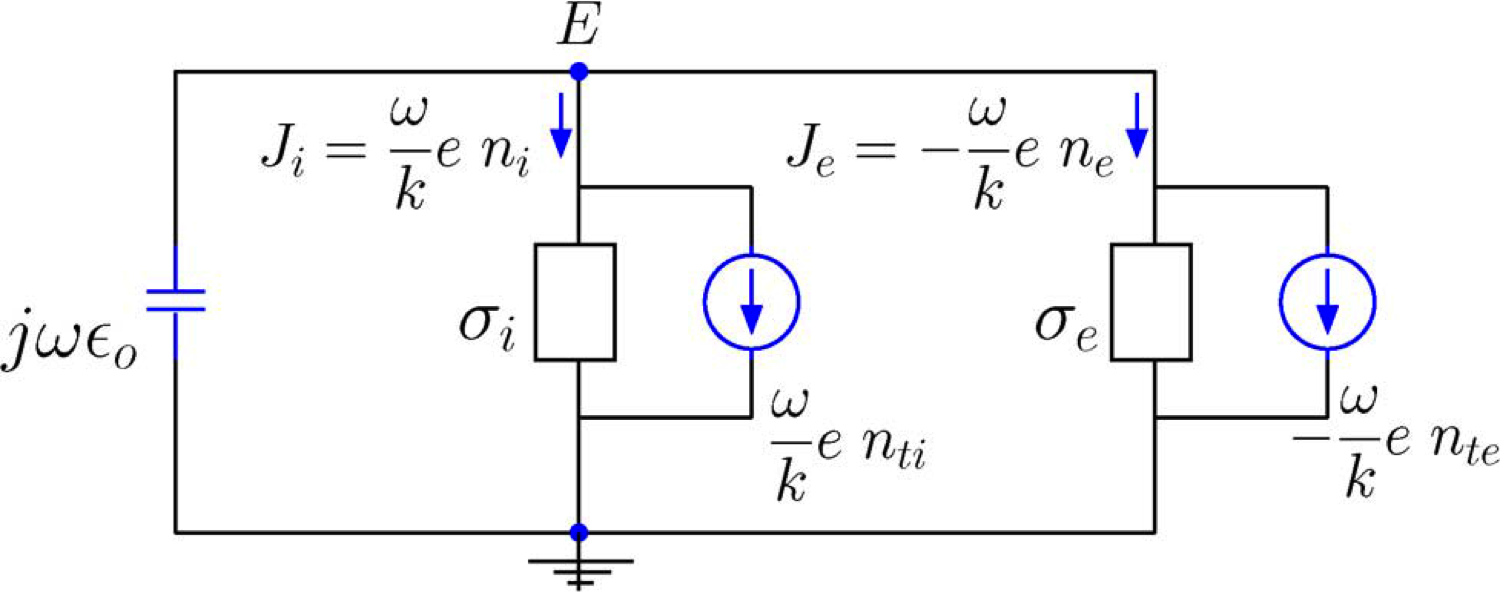
\includegraphics[width=3.0in]{circuit}
% where an .eps filename suffix will be assumed under latex, 
% and a .pdf suffix will be assumed for pdflatex; or what has been declared
% via \DeclareGraphicsExtensions.
\caption{Lumped circuit model seen in  \cite{kudeki:milla:1}.}
\label{fig:circuit}
\end{figure}

\noindent Using the electron current expression, $-\omega k^{-1}en_e = E\sigma_e -\omega k^{-1}en_{te}$, these equations can be rearranged to solve for $n_e$, 

\begin{equation}
\label{eq:neeq}
n_e(\mathbf{k},\omega) =  \frac{(j\omega\epsilon_0 + \sigma_i) n_{te}(\mathbf{k},\omega)}{j\omega\epsilon_0 +\sigma_e+\sigma_i} + \frac{\sigma_en_{ti}(\mathbf{k},\omega)}{j\omega\epsilon_0 +\sigma_e+\sigma_i}.
\end{equation}

\noindent To determine the power spectrum we square and average Equation \ref{eq:neeq} taking into account that the terms $n_{te}$ and $n_{ti}$ are independent of one and other we result in the following
\begin{equation}
\label{mainspeceq}
\langle \left|n_e(\mathbf{k},\omega)\right|^2\rangle = \frac{|j\omega\epsilon_0 + \sigma_i|^2 \langle |n_{te}(\mathbf{k},\omega)|^2\rangle}{|j\omega\epsilon_0 +\sigma_e+\sigma_i|^2} + \frac{| \sigma_e|^2 \langle |n_{ti}(\mathbf{k},\omega)|^2\rangle}{|j\omega\epsilon_0 +\sigma_e+\sigma_i|^2}.
\end{equation}

We can generalize them for multiple ion species by simply summing over the thermal fluctuations and conductances in Equation \ref{eq:ampscaler},

\begin{equation} 
\label{eq:ampscalersum}
0=\left(\displaystyle \sum_k^K\sigma_{ik} +\sigma_e\right)E +\frac{\omega}{k}e\left(\sum_k^Kn_{tik}-n_{te}\right) +j\omega \epsilon_0 E.
\end{equation}

\noindent This then augments the power spectrum in Equation \ref{mainspeceq} to the following

\begin{equation}
\label{eq:sumspeceq}
\displaystyle \langle \left|n_e(\mathbf{k},\omega)\right|^2\rangle = \frac{\left|j\omega\epsilon_0 +  \sum_k^K\sigma_{ik} \right|^2 \langle |n_{te}(\mathbf{k},\omega)|^2\rangle}{\left|j\omega\epsilon_0 +\sigma_e+ \sum_k^K\sigma_{ik} \right|^2} + \frac{| \sigma_e|^2 \left \langle \left|\sum_k^Kn_{tik}(\mathbf{k},\omega)\right|^2\right\rangle}{\left|j\omega\epsilon_0 +\sigma_e+ \sum_k^K\sigma_{ik} \right|^2}.
\end{equation}

%%%%%%%%%%%%%%%%%%%%%%%%%%%%%%%%%%%%%%%%%%%%%%%%%%%%%%%%%%%%%%%%%%%%%%
\section*{Gordeyeve Integrals}
The power spectrum of the thermal fluctuation for each species $s$ can be determined by the following,

\begin{equation}
\label{eq:thermalfl}
\frac{\langle|n_{ts}(\mathbf{k},\omega)|^2\rangle}{N_0} = 2\text{Re}\{J_s(\omega_s)\},
\end{equation}

\noindent where $N_s$ is the average density for the species.  Also the conductance for each species $s$ can be determine from the following,

\begin{equation}
\label{eq:cond}
\frac{\sigma_{s}(\mathbf{k},\omega)}{j\omega\epsilon_0} = \frac{1-j\omega_s J_s(\omega_s)}{k^2\lambda_s}
\end{equation}

\noindent where $\omega_s \equiv \omega-\mathbf{k}\cdot\mathbf{V}_s $ is the Doppler shifted frequency and $\lambda_s \equiv \sqrt{\frac{\epsilon_0 KT_s}{N_s q_s^2}}$ is the Debye length for each species.

The $J_s$ terms can be represented as follows

\begin{equation}
\label{eq:gord}
J_s(\omega)\equiv \int_0^\infty \langle e^{j\mathbf{k}\cdot\Delta \mathbf{r}_s}\rangle e^{j\omega\tau}d\tau
\end{equation}

\noindent These terms are known as Gordeyeve integrals, which are the one sided Fourier transforms of the characteristic functions of the particle displacements $\langle e^{j\mathbf{k}\cdot\Delta\mathbf{r}_s}\rangle$.  

The particle displacement function can change depending on magnetic field and collisionality of the plasma. For the high latitude F-region in the ionosphere a case of general importance is one of a non-magnitized and collision less plasma, where $\Delta\mathbf{r} = \mathbf{v}\tau$ where $\tau$ is the time interval. Assuming a Maxwellian the PDF of one dimensional displacement is

\begin{equation}
\label{eq:pdfr}
f(\Delta r) = \frac{1}{\sqrt{2\pi \langle r^2 \rangle}}e^{\frac{-\Delta r^2}{2\langle r^2\rangle}}.
\end{equation}
 
\noindent The variance term $\langle r^2 \rangle$ can be represented as
\begin{equation}
\label{eq:var}
\langle r^2 \rangle = \langle v^2 \rangle \tau^2 = \frac{KT_s}{m_s} \tau^2
\end{equation}
 \noindent where $T_s$ is the temperature of the species, $K$ is Boltzmans constant and $m_s$ is the mass of the species in kg. To simplify notation like in \cite{kudeki:milla:1}, we will refer to $\sqrt{KT_s/m_s}$ as $C$. Which yields the following single particle ACF,
 
 \begin{equation}
\label{eq:pdfall}
\langle e^{j\mathbf{k}\cdot\Delta \mathbf{r}}\rangle= e^{-\frac{1}{2}k^2C^2 \tau^2}.
\end{equation}
 
 To model collisions we use the term $\nu$ as the collision frequency for the species. If $\nu<<kC$ then \ref{eq:pdfall} can be used as the single particle ACF. If not the following must be used.
 
 \begin{equation}
 \label{eq:colspacf}
 \langle e^{j\mathbf{k}\cdot\Delta \mathbf{r}}\rangle = e^{-\frac{k^2C^2}{\nu^2}\left( \nu \tau-1+e^{-\nu\tau}\right)}
 \end{equation}
 
Lastly if one is to add a magnetic field to the equations the single particle ACFs must now take into a account the orientation of the magnetic field. The authors of \cite{kudeki:milla:1} use the convention of breaking up the Bragg vector $\mathbf{k}$ into two components, one parallel to the magnetic field, $k_{\parallel}$ and one perpendicular,$k_{\perp}$, as such, $\mathbf{k}= \hat{b}k_{\parallel}+\hat{p}k_{\perp}$. This yields the following formulation for the single particle ACF,

 \begin{equation}
\label{eq:pdfmag}
\langle e^{j\mathbf{k}\cdot\Delta \mathbf{r}}\rangle= e^{-\frac{1}{2}k_{\parallel}^2C^2 \tau^2}\times e^{-\frac{2k_{\perp}^2C^2}{\Omega^2} \sin^2(\Omega\tau/2)},
\end{equation}

\noindent where the gyro frequency is $\Omega = qB/m$This formulation neglects the effects of collisions which if taken into account yields the following single particle ACF,

\begin{equation}
\label{eq:colspacf}
\langle e^{j\mathbf{k}\cdot\Delta \mathbf{r}}\rangle = e^{-\frac{k_\parallel^2C^2}{\nu^2}\left( \nu \tau-1+e^{-\nu\tau}\right)}\times e^{-\frac{k_\perp^2C^2}{\nu^2+\Omega^2}\left(\cos(2\gamma) + \nu \tau-e^{-\nu\tau}\cos(\Omega\tau-2\gamma)\right)},
\end{equation}
 
\noindent where $\gamma = \tan^{-1}(\nu\Omega)$. The for the case with the magnetic field as one gets closer to being fulling perpendicular to $\mathbf{B}$ the single particle ACFs become much more narrow band, to the point of becoming delta functions in the frequency space. It is necessary to use other methods beyond numerical integration to determine the Gordeyeve Integrals. The authors of \cite{kudeki:milla:2} get around this problem by making a PIC code to determine the particle statistics. 
%%%%%%%%%%%%%%%%%%%%%%%%%%%%%%%%%%%%%%%%%%%%%%%%%%%%%%%%%%%%%%%%%%%%%%
 \section*{Computational Considerations}
One of the main challenges to calculating the ISR spectrums is calculating the Gordeyeve integrals. The case with no collisions or magnetic fields can be done analytically using Dawsons integral. This can be done using the identity

\begin{equation}
\label{eq:daw1}
jZ(\theta) = \int_0^{\infty} e^{-j\theta t}e^{-\frac{t^2}{4}}dt = \sqrt{\pi}e^{-\theta^2}-j2e^{-\theta^2}\int_0^\theta e^{t^2}dt.
\end{equation}

\noindent Using the terms found in Equation \ref{eq:pdfall}, $\theta=\omega_s/\left(\sqrt{2}kC\right)$ and $t=\sqrt{2}kC\tau$.

For other cases where analytical calculation is not possible a numerical integration scheme from \cite{Ooi:2007jx} is used. It is also possible to use a Chirp-z based algorithm that is shown in \cite{Li:1991gr} from the experiences of the author the first technique converges faster. The technique used in \cite{Ooi:2007jx} changes the variable of integration for integrals of the following form,

\begin{equation}
\label{eq:Sommer}
I=\int_a^b f(z) dz.
\end{equation}

\noindent The technique changes the variable $z$ in the following way,

\begin{equation}
\label{eq:newz}
z = \frac{1}{2}(a+b)+\frac{1}{2} (b-a)\text{Erf}(g(t)),
\end{equation}

\noindent where $g(t)$ is a function that is choosen so  $g(t)\rightarrow\pm \infty$ as $t\rightarrow\pm \infty$ and $Erf(u)$ is 
\begin{equation}
\label{eq:erf1}
\text{Erf}(u) = \frac{2}{\sqrt{\pi}}\int_0^u e^{-t^2}dt.
\end{equation}

\noindent Discretizing and changing variables the integral in Equation \ref{eq:Sommer} becomes the following sum

\begin{equation}
\label{eq:erfsum1}
I=\displaystyle \sum_{n=-N}^N A_nf\left( \frac{1}{2}(a+b)+\frac{1}{2} (b-a)\text{Erf}(g(nh))\right)
\end{equation}

\noindent where,
\begin{equation}
\label{eq:anterm}
A_n = g'(nh)e^{-g(nh)^2}.
\end{equation}

\noindent Like in \cite{Ooi:2007jx}, $g(nh) = \sinh (nh)$ and the grid spacing $h$ is the following,

\begin{equation}
\label{eq:hterm}
h = \frac{1}{N}\ln(1.05\sqrt{2}N).
\end{equation} 


Lastly to avoid cases of divid by zero errors the main equations have to be rearrange slightly. First off because some ion species could have zero density Equation \ref{eq:cond} uses the Debye length of the electron species,$\lambda_e$ as follows

\begin{equation}
\label{eq:condnew}
\frac{\sigma_{s}(\mathbf{k},\omega)}{j\omega\epsilon_0} = \frac{1-j\omega_s J_s(\omega_s)}{k^2\lambda_e} \left(\frac{q_sT_eN_s}{q_eT_sN_e}\right).
\end{equation}

Also, to avoid having to more calculations then necessary the $j\omega\epsilon_0$. terms of Equation \ref{eq:sumspeceq} are moved around. Thus it becomes,

\begin{equation}
\label{eq:sumspeceqfinal}
\displaystyle \langle \left|n_e(\mathbf{k},\omega)\right|^2\rangle =  \frac{\left|1 +  \sum_k^K\frac{\sigma_{ik}}{j\omega\epsilon_0} \right|^2 \langle |n_{te}(\mathbf{k},\omega)|^2\rangle}{\left|1 +\frac{\sigma_e+ \sum_k^K\sigma_{ik}}{j\omega\epsilon_0} \right|^2} + \frac{\left| \frac{\sigma_e}{j\omega\epsilon_0} \right|^2\left \langle \left|\sum_k^Kn_{tik}(\mathbf{k},\omega)\right|^2\right\rangle}{\left|1 +\frac{\sigma_e+ \sum_k^K\sigma_{ik}}{j\omega\epsilon_0} \right|^2}.
\end{equation}



\chapter{Data Formation}
The 3-D ISR simulator creates data by deriving a time filter from the autocorrelation functions and applying them to complex white Gaussian noise generators. Stating this in another way, every point in time and space has a noise plant and filter structure as in Figure \ref{fig:IQdiagram}. The data is then scaled and summed together according to its location in range and angle space to radar. For this simulation, data points are only used if they are within 1.1 $^\circ$ of the center beam which is a simplification of the AMISR beam pattern. 

\begin{figure}[h!]
\centering
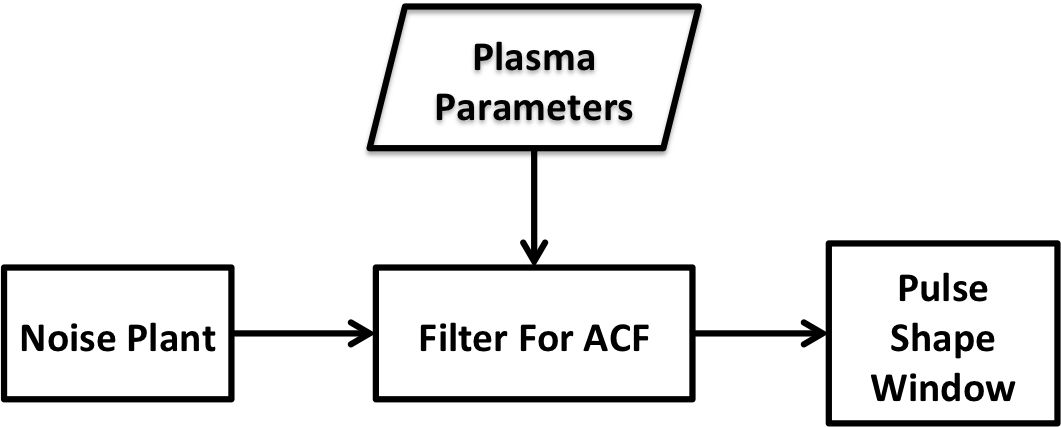
\includegraphics[width=4in]{diagrampart}
\caption{Diagram for I/Q simulator signal flow.}
\label{fig:IQdiagram}
\end{figure}

After the IQ data has been created it is processed to create estimates of the ACF at desired points of space. This processing follows a flow chart seen in Figure \ref{fig:chain}.

\begin{figure}[!t]
\centering
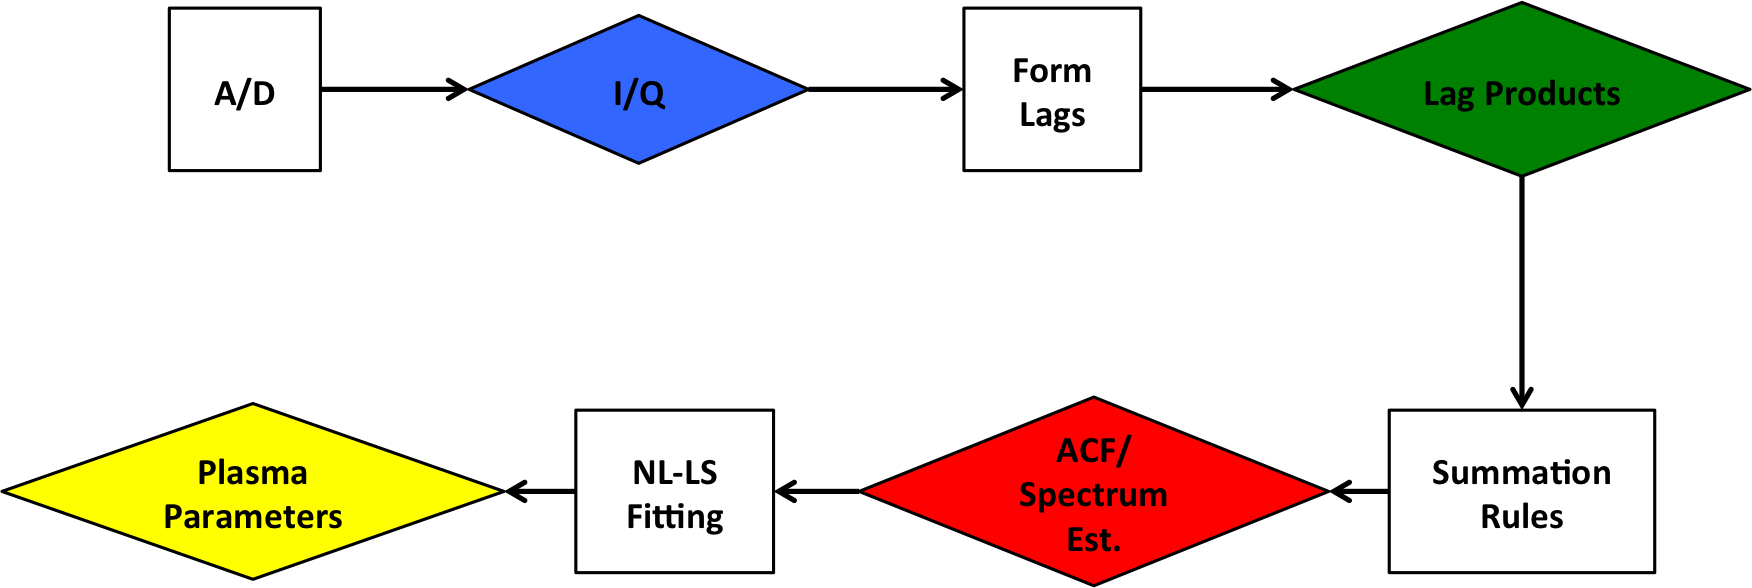
\includegraphics[width=6in]{datastackchain}
\caption{ISR signal processing chain, with signal processing operations as squares and data products as diamonds.}
\label{fig:chain}
\end{figure}

\chapter{ISR Processing}

The sampled I/Q voltages can be represented as $x(n_s) \in\mathbb{C}^N$ where $N$ is the number of samples in a PRI.  At this point, the first step in estimating the autocorrelation function is taken.  For each range gate $m\in 0,1,...M-1$ an autocorrelation is estimated for each lag of $l \in 0,1...,L-1$.  This operation of forming the ACF estimates repeats for each pulse, $j\in 0,1,...J-1$, and is then summed over the $J$ pulses. The entire operation to form the initial estimate of $\hat{R}(m,l)$ is the following,

\begin{equation}
\label{lagpro}
\hat{R}(m,l) = \displaystyle\sum\limits_{j=0}^{J-1} x(m-\lfloor l/2\rfloor,j)x^*(m+\lceil l/2 \rceil,j).
\end{equation}


The case shown in Equation  \ref{lagpro} is a centered lag product, which is what has been used for our simulations, but other types of lag product calculations are possible as well. In the centered lag product case, range gate index $m$ and sample index $n$ can be related by $m=n_s-\lfloor L/2\rfloor$ and the maximum lag and sample relation is $M=N-\lceil L/2 \rceil$. 

After the lag products have been formed, an estimate of the noise correlation is subtracted out of $\hat{R}(m,l)$, defined as $\hat{R}_w(m,l)$,

\begin{equation}
\label{lagpronoise}
\hat{R}_w(m_w,l) = \displaystyle\sum\limits_{j=0}^{J-1} w(m_w-\lfloor l/2\rfloor,j)w^*(m_w+\lceil l/2 \rceil,j),
\end{equation}

\noindent where $w(n_w)$ is the background noise process of the radar. 

The final estimate of the autocorrelation function after the noise subtraction and summation rule will be represented by $\hat{R}_f(m,l)$. At this point, a summation rule is applied and the data is sent off to be fit. The final parameters are derived through fitting these estimated ACFs with a standard Levenberg-Marquardt non-linear least-squares algorithm \cite{levenberg1944}, to ones that are determined using a theoretical model of the plasma ACF after application of the range ambiguity function. The simulations presented in this work use this methodology to produce plasma parameter scalar values of electron density, electron temperature, and ion temperature. To plot the three dimensional structures after fitting, we use a natural neighbor interpolation as seen in \cite{Semeter2009738}.


 \bibliographystyle{BibTeX/ieeetrsrt}

 \bibliography{BibTeX/litreview}

 \end{document}